
%%%%%%%%%%%%%%%%%%%%%%% file typeinst.tex %%%%%%%%%%%%%%%%%%%%%%%%%
%
% This is the LaTeX source for the instructions to authors using
% the LaTeX document class 'llncs.cls' for contributions to
% the Lecture Notes in Computer Sciences series.
% http://www.springer.com/lncs       Springer Heidelberg 2006/05/04
%
% It may be used as a template for your own input - copy it
% to a new file with a new name and use it as the basis
% for your article.
%
% NB: the document class 'llncs' has its own and detailed documentation, see
% ftp://ftp.springer.de/data/pubftp/pub/tex/latex/llncs/latex2e/llncsdoc.pdf
%
%%%%%%%%%%%%%%%%%%%%%%%%%%%%%%%%%%%%%%%%%%%%%%%%%%%%%%%%%%%%%%%%%%%


\documentclass[runningheads,a4paper]{llncs}

\usepackage{amssymb}
\setcounter{tocdepth}{3}
\usepackage{graphicx}
\usepackage{verbatim}%长篇注释宏包
\usepackage{mathrsfs}
\usepackage{mathtools}
\usepackage{multirow}
\usepackage{cite}
\usepackage{amsmath}
\usepackage{amsmath}
\usepackage{amssymb}
\usepackage{url}
\urldef{\mailsa}\path|{alfred.hofmann, ursula.barth, ingrid.haas, frank.holzwarth,|
\urldef{\mailsb}\path|anna.kramer, leonie.kunz, christine.reiss, nicole.sator,|
\urldef{\mailsc}\path|erika.siebert-cole, peter.strasser, lncs}@springer.com|    
\newcommand{\keywords}[1]{\par\addvspace\baselineskip
\noindent\keywordname\enspace\ignorespaces#1}


\newcommand{\reffig}[1]{Fig. \ref{#1}}
\newcommand{\refsec}[1]{Section \ref{#1}}
% \newcommand{\refeq}[1]{Eq. \ref{#1}}
\newcommand{\reftab}[1]{Table \ref{#1}}


\DeclareMathOperator*{\argmax}{argmax}
\DeclareMathOperator*{\argmin}{argmin}



\begin{document}

\mainmatter  % start of an individual contribution

% first the title is needed
\title{Background Subtraction via Deep Variation Transformation}

% a short form should be given in case it is too long for the running head
 \titlerunning{Background Subtraction via Deep Variation Transformation}

% the name(s) of the author(s) follow(s) next
%
% NB: Chinese authors should write their first names(s) in front of
% their surnames. This ensures that the names appear correctly in
% the running heads and the author index.
%i
\author{Yongxin Ge, Xinyu Ren, Chenqiu Zhao}
%
\authorrunning{Lecture Notes in Computer Science: Chongqing University}
% (feature abused for this document to repeat the title also on left hand pages)

% the affiliations are given next; don't give your e-mail address
% unless you accept that it will be published
\institute{Laboratory of Intelligent Services and Software Engineering, \\
School of Software Engineering,\\
Chongqing University, Chongqing 401331, China\\
\url{xxx@cqu.edu.cn}}

%
% NB: a more complex sample for affiliations and the mapping to the
% corresponding authors can be found in the file "llncs.dem"
% (search for the string "\mainmatter" where a contribution starts).
% "llncs.dem" accompanies the document class "llncs.cls".
%

\toctitle{Lecture Notes in Computer Science}
\tocauthor{Chongqing University}
\maketitle


\begin{abstract}
%Background subtraction in complex scenes is a challenging problem
One of the main challenges of foreground detection comes from the diversity and complexity of real-world scenes. While most of previous works in this field were proposed by designing an artificial model, we tend to present a self-adaption solution, by combining the fully convolutional networks (FCNs), which is named as the Deep Pixels Variation Learning model (DPVL). Our main job is to find a new representation of pixels historical observations in a new feature space. In this paper, videos are divided into fixed length image stacks, which are later transformed into the pixel observation matrixes as the input of a FCN for learning the variation of pixels. We conduct our training and prediction processes on stack level. The architecture of the FCN is devised from the semantic segmentation problem. Experiment shows that our model has a strong learning ability to the patterns of those permutations of pixels’ variation. We compare our method with some state-of-the-art methods, and the results show that the proposed approach outperform its
\keywords{Background Subtraction, Motion Detection, Superpixels, Neighborhood Information, Multi-Scale}
\end{abstract}

\section{Introduction}
% 问题的意义
背景建模一直都是视频分析的基础,不仅可以帮助研究人员在视频中提取出感兴趣区域,其在现实生活中也有着广反的应用,

Background subtraction is a fundamental issue of computer vision,
which has a wide range of application \cite{2014_CSR_reviews} \cite{2014_CCPR_RefPaper}.
% 问题的挑战
在这个问题中,主要的挑战来自于运动物体的运动模式难以预测,以及野外的复杂动态背景,例如流动的水和摇晃的树木。
The main challenge in background subtraction comes from the complexity
of nature scenes, such as waving tree or rippling water.
% previous work
绝大多数现有的方法都是
Recently, large numbers of works used pixels' neighborhood information to
improve the robustness of background subtraction.
% 这些方法的缺点
Unfortunately, most of those algorithms were based on pixels or regions and
ignored the similarity between pixels themselves.
% 一个像素,有很多邻居,以前的方法把所有的都用上了
And those pixels or regions based algorithms utilize the information of all
pixels' neighborhoods.
% 像素的相似度是不同的,不是所有的像素,都是正面影响
However, since the similarity between a pixel and their neighborhoods is
different,
%
not all pixels' neighborhoods contribute positively to improve the robustness of algorithms.
% 我们的思路
In this work, the superpixel contains the pixels'
neighborhood information as well as the similarity among them is utilized to
detect moving objects.
% 具体的方法
And a novel background subtraction based on superpixels under multi-scale is
proposed to background subtraction in complex scenes.

% 从描述现象开始
Background subtraction is the classification of pixels according its variation.
% 开始描述图
Since the complexity of natural scenes, several pixels with different labels have the
similar variation.
% 左边的图混合在一起
For example, as the left part of \reffig{thinking} shows, the pixels labeled as
foreground or background are mixing together in the variation of RGB space.
% 
However, a pixel is not independent \cite{2009_ICASSP_ViBe} but related
with its neighborhoods, especially the similar one.
% 
Since the superpixels contain the information on pixels and their similar neighborhoods, the variation in
the superpixels is easier to be classified, such as the right part
of \reffig{thinking} shows.
% 
Unlike previous work, we analyze the variation in superpixels instead of pixels for
background subtraction.
% 超像素只能把物体分开,不能确定哪里是前景
Moreover, since the segmentation of superpixels does not refer to motion
information, not all the pixels belong to a particular superpixel are shared
the same label of foreground or background.
% 为了解决这个被引入的问题,用了一个多尺度的方法
To solve this brought issue, the labelled superpixels are obtained under
multiple scales to compose different foreground in each scale.
% 我们的前景是怎么由这个方法得到的
And the final foreground of our SPMS is captured by the summary of several foregrounds
consisted of superpixels under different scales.
\begin{figure}
    \centering
    \includegraphics[width=\textwidth]{figure/fig_idea}
    \caption{The variation in pixels and superpixels with foreground or background labels.}
    \label{thinking}
\end{figure}

% 我们方法的具体细节
Our SPMS method can be divided into three step.
% 跟以前的方法一样,获取背景图像
The first step of SPMS is learning a background via the statistical function such as
Gaussian function \cite{1997_TPAMI_GAUSS}.
% 超像素获取的方法
Meanwhile, the current frame is segmented into several superpixels by a
\emph{K-means} based superpixel segmentation algorithm \cite{2012_TPAMI_SLIC}.
% 相减获得每一个的变化
Then, we subtract the current frame and background to capture the variation of each pixel.
% 统计变化,得到superpixel的变化
And the means of pixels' variation in a particular superpixel is used as the
variation in it.
% 变化直接二值化
The variation is classified by a threshold to decide whether it
is foreground or background.
% 标记好的超像素为SPMS的foreground
And the foreground of SMPS is consisting of these labeled superpixels in a
particular scale.
% 使用了多尺度
Finally, the segmentation of foreground in SPMS is done under multiple scales.
% 多尺度里超像素尺寸不同
We modify the size and zone of superpixels in each scale to capture different foregrounds.
% 最终的目的
And the summary of these foregrounds under different scales is used as our final
foreground result.
% 论文的贡献
The contributions of this paper are summarized as follows:
\begin{enumerate}
    \item Our SPMS utilizes superpixels instead of pixels or regions for
        background subtraction. Since the superpixel reveals the neighborhood
        information and the similarity among pixels, proposed approach achieves
        encouraging robustness in complex scenes, such as adverse weather and
        dynamic scene.
    \item The final foreground of SPMS is captured by the summary of
        foregrounds captured in different scales. Benefited from the difference
        about superpixels' zone in multiple scales, the accuracy of our SPMS
        background model is improved by the summary process.
\end{enumerate}

\section{Related Work}
% 引子,简单介绍不利用领域信息的方法
In the early works about background subtraction, pixels are assumed independent
of each other.
The MoG \cite{1997_TPAMI_GAUSS} \cite{1999_CVPR_MoG} and the CodeBook
\cite{2004_ICIP_CodeBook} \cite{2006_RTI_CodeBook} algorithms are two
popular approaches to segment foreground.
% 以前方法的没有考虑的东西
However, since those works ignored the neighborhood information, both
the MoG \cite{1999_CVPR_MoG} and CodeBook \cite{2006_RTI_CodeBook} are
working hard in complex scenes, like waving tree and rippling water.

% 近期的工作开始利用领域信息
Recently, larger numbers of works improved the robustness of background
subtraction by neighborhood information (e.g. \cite{2010_CVPR_SILTP},
\cite{2014_IS_MulLevTex}, \cite{2009_ICASSP_ViBe}, \cite{2011_TIP_ViBep},
\cite{2012_CVPRW_ViBe_Van}, \cite{2006_TPAMI_TexBased},
\cite{2014_TIP_Spatio_Lin} and \cite{2011_ICCV_MultiScale_Zaharescu}).
% 引子
Among those works, several algorithms are based on features with
neighborhood information.
% 蕴含领域信息的特征 texture
Heikkila et al. \cite{2006_TPAMI_TexBased} modeling the background by LBP
\cite{2006_TPAMI_TexBased} texture descriptor, which is captured from pixels
and its neighborhoods.
% 论文的好处
Since the LBP is robust to illumination change and noise, the algorithm
in \cite{2006_TPAMI_TexBased} work well in the shade regions.
% 增强算法
Similarly, Liao et al. \cite{2010_CVPR_SILTP} improved the LBP into SILTP and
segmented the foreground by Kernel Density Estimation.
% multilevel
Hence, Lin et al. \cite{2014_IS_MulLevTex} detected moving objects in different levels
to improve the efficiency of their algorithm.
% multi-scale codebook
And Zaharescu et al. \cite{2011_ICCV_MultiScale_Zaharescu} extended the
CodeBook algorithm by multiple scales for the accuracy of
foreground.

% the spatio-temporal features
Besides the texture features, the spatio-temporal features (e.g.
\cite{2014_TIP_Spatio_Lin} and \cite{2014_ICIP_MultiScaleSpatio_Lu}) also
reveals the neighborhood information.
% the pursuing dynamic spatio-temporal
Lin et al. \cite{2014_TIP_Spatio_Lin} detect moving objects by pursuing dynamic
spatio-temporal model.
They employed the auto regressive moving average model
to pursue the subspace. And model joints the appearance consistency and temporal
coherence of the observations.
% multiscale spatioi
Lu et al. \cite{2014_ICIP_MultiScaleSpatio_Lu} collected a set of samples on
different spatial scales for each location in a dynamic scene. And the
foreground is segmented by a non-parametric model.
% ViBe and ViBe++
Barnich et al. proposed the ViBe \cite{2009_ICASSP_ViBe} and ViBe+
\cite{2011_TIP_ViBep} algorithm, which is an excellent method to utilize
neighborhood information.
% ViBe 具体的做法
The ViBe algorithm maintains a sample set,which contains
the pixels and their neighborhoods, for each pixels.
And the pixel is label as background if it is matched with
any entries of the sample set.
% histogram
In addition, the histogram is another technique of the
utilization about neighborhood information.
% Background modeling by combining joint intensity histogram with time-sequential data
Kita et al. \cite{2010_ICPR_KitaHis} segmented foreground by analysing the
intensity histogram during video sequence. And a similar method also based on
histogram is proposed in \cite{2009_ICIC_KuoHis}.
% 我们方法与它们的区别

% the region based algorithms
Furthermore, these are also several works detected moving objects by regions
instead of pixels.
% rect gauss
Riahi et al. \cite{2012_PD_RECTGAUSS} extended the MoG with rectangle region.
Since the variation in the regions' intensity is robust to environment
change, the algorithm in
\cite{2012_PD_RECTGAUSS} achieves well performance in complex scenes.
% regions-based spatio-temporal features
Varadarajan et al. \cite{2013_AVSS_RMoG_Varadarajan} proposed a
region-based MoG algorithm. In particular, the spatio-temporal features
is extracted from the regions and as the input of MoG to segment
foreground.
% XXX 解释和区域方法的不同
The main difference between our work and regions based algorithms is the consideration of similarity between pixels themselves.
% 
The pixels in a superpixel have stronger connection with each others compared with pixels in a region.
%
And the stronger connection prevents the accuracy of our superpixel-based approach.

% 超像素
One should note, the superpixels also utilized for background subtraction in
several algorithms (e.g. \cite{2014_CVPR_Superpixel_Zhu},
\cite{2008_TPAMI_PixelLayers_Patwardhan}, \cite{2015_TCSVT_Reshape_Wu}).
% pixels layers
In the \cite{2008_TPAMI_PixelLayers_Patwardhan}, Patwardhan et al.
\cite{2008_TPAMI_PixelLayers_Patwardhan} cluster pixels into several pixel
layers. And the foregrounds are segmented from different pixel layers.
% reshape the foreground
Moreover, Wu et al. \cite{2015_TCSVT_Reshape_Wu} detect moving objects by
the trajectory, and reshape the foreground by superpixels.
% superpixel
In addition, proposed approach is closely related with the work in
\cite{2014_CVPR_Superpixel_Zhu}, which is a saliency detection algorithm.
However, besides the difference in purpose, the similarity measure also
different between us.
The algorithm in \cite{2014_CVPR_Superpixel_Zhu} just
threshold the gray-scale of current frames. And in this work, the similarity of
superpixels is captured by the analysing of its variation during time sequence.

\section{Modeling Background by Superpixels}
\label{model_SPMS}
In this section, the details of SPMS model are explained and its flow chart is
shown in \reffig{flow_chart}
% 总结这段的作用,而且要以本文的方法总结,来突出我们方法的新异
In the \refsec{model_segmentation}, we introduce the segmentation of foreground
via analysing the variation of superpixels' intensity under multi-scale.
% 解释背景的作用,已经背景的更新
Simultaneously, the process of capturing background, which is used to compare
with current frame for extracting superpixels' variation, is explained in
\refsec{model_update}.

\subsection{Foreground Segmentation via Superpixels under Multi-Scale}
\label{model_segmentation}
% 前景是由带标签的超像素组成的
In our SPMS model, the foreground consists of superpixels with foreground or
background label.
% 超像素的标签是由背景和当前帧对比得到
The label of each superpixel is decided by its variation.
% variation 怎么得的
And the variation in a superpixel is actually the means of their pixels'
variation compared with the corresponding pixels in the background.
% Backgroudn
In particular, the process of capturing background will be explained later.
% 多尺度的怎么用的
Moreover, in order to improve the accuracy of proposed approach, we segment
several foregrounds under multiple scales, and the summary of all these
foreground information is used as the final result of proposed approach.

\begin{figure}
    \centering
    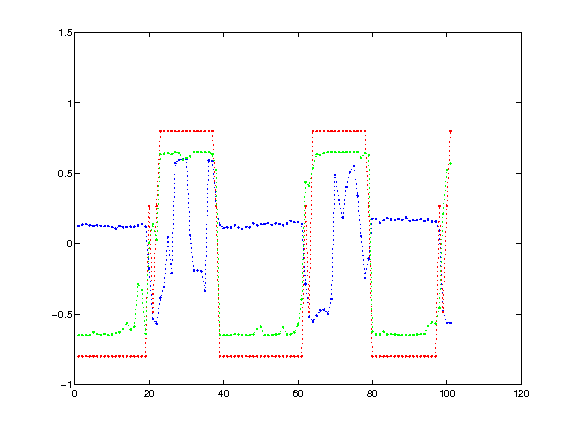
\includegraphics[width=\textwidth]{figure/fig1}
    % XXX 图例里描述一下。
    \caption{The pipeline of proposed approach.}
    \label{flow_chart}
\end{figure}
% 超像素获取的方法
In this work, the superpixel are obtained from current frame by the SLIC algorithm \cite{2012_TPAMI_SLIC}.
% 这个方法的特
Since the SLIC \cite{2012_TPAMI_SLIC} is based on \emph{K-Means}, it is
convenient to control the size of superpixels according to the numbers.
%
And the convenience is the main reason we choose SLIC algorithm
\cite{2012_TPAMI_SLIC}.
% 假设超像素的公式
Let's denote the superpixels segmented under multi-scale are:
\begin{equation}
\{\mathcal{SP}_1,
\mathcal{SP}_2, \dots \mathcal{SP}_s \} = \{ Sp_{i,j}|i \in [1,s], j \in [1,N_i] \},
\end{equation}
where $i$ is the index of scale and $N_i$ is the number of superpixels under scale $i$.

% 最后的前景是综合得到
As we mentioned before, the final foreground is captured by the summary of
foregrounds segmented under multiple scales.
% 每一个前期是怎么得到的
And the foreground in each scale consists of superpixels with foreground or
background segmented under this scale.
% 解释一个超像素
In the superpixel $Sp_{i,j}$, all their pixels are subtract from
pixels of background $I_b(x,y)$ in the corresponding position.
% 解释相减的细节
Moreover, in the subtracting process, we utilized a region searching method to
improve the robustness of the subtraction result.
% 
In the region searching method, for each a pixel, we find the most similar pixels of
background in a small region $R$ on respective position of it.
% 公式表达
And the definition of region searching method $G(x,y)$ is shown as follows:
\begin{equation}
    G(x,y) =  \mathop{\argmin}_{}{ \lVert I_t(m,n) - I_b(x,y) \rVert_{1}  } \quad  m,n \in x,y \pm R,
\end{equation}
where $x$ and $y$ is the location of pixels. And $I_t$ is the current frame, where $t$ is the
time index.

% 解释超像素的相似度
Then, the score of this superpixel labelled as background is captured from the
means of all the subtraction results on it, which is shown as follows:
\begin{equation}
    P(Sp_{i,j}) = \quad \frac{ \sum\limits_{ \mathclap{x,y \in Sp_{i,j}} }G(x,y)}{|Sp_{i,j}|} ,
\end{equation}
where $N_i$ is the number of pixels belong to superpixel $Sp_{i,j}$, and
$G(x,y)$ is the similarity function of position $(x,y)$. The $P(Sp_{i,j})$ is
compared with a threshold $T_{sp}$ to decide whether the superpixel $Sp_{i,j}$
is foreground or background. And foreground of our SPMS under a particular
scale $i$ consists of all the labelled superpixels. And the process is shown as
follows:
\begin{equation}
    Fg_{i}(x,y) = g(Sp_{i,j}(x,y),T_{sp}), \quad I_t(x,y) \in Sp_{i,j},
\end{equation}
where $g(x,y)$ is the piecewise function to decide whether the pixel with
location $(x,y)$ is foreground or background, and the definition is shown as
follows:
\begin{equation}
    \label{piecewise_fg}
    g(x,y) =
 \begin{cases}
  1,  \quad x < y       \\
  0,  \quad otherwise   \\
\end{cases}.
\end{equation}

The superpixel is the set of similar pixels and does not consider motion
information. Background subtraction based on superpixel achieves well
robustness but suffer from accuracy problem. We captured foregrounds
under different scales. The summary of all these foregrounds improve the
accuracy of proposed approach, which is defined as:
\begin{equation}
    Fg(x,y) = \frac{ \sum\limits_{i = 0}^{s}Fg_i(x,y)}{s}
\end{equation}
where $Fg(x,y)$ is the proximity image of SPMS and is utilized to compare
with threshold $T$ for our final foreground segmentation.

\subsection{Background Updating}
\label{model_update}
% 背景更新的目的是为了得到一个没有前景的图像
The purpose of background updating is to capture a background without
moving objects.
% 背景会更新去适应场景变化
The updating procedures are different to the pixels labeled as foreground and background.
%
If a pixel is labelled as background in the procedure of foreground segmentation.
%
The respective pixel in background is replaced by this pixel.
%
When a pixel is labeled as foreground, the process shown in
\reffig{fig_bkupdate} is done to capture the background intensity.
%
And the background intensity is used to update the pixel with the corresponding
location in the background.
% 背景是怎么得到的
\begin{figure}
    \centering
    \includegraphics[width=\textwidth]{figure/fig5}
    \caption{The process of updating foreground is analysing the variation of
    pixels' intensity.}
    \label{fig_bkupdate}
\end{figure}

% 总结fig中的过程
The procedure shown in \reffig{fig_bkupdate} is a histogram of the pixel's
variation during time sequence.
Let's denote the observation of a pixel labeled as foreground in time sequence as $P = {p_1,p_2,\dots,p_t}$.
The variation of this pixel is analyzed by the histogram.
and the intensity with the max peak value is used as the
background intensity. Mathematically, the background intensity is defined as:
\begin{equation}
    p_{bk} = \mathop{\argmax}_{p}{\sum\limits_{i = 1}^{t} p_i \cap p} \quad p = \{p_1,p_2,\dots,p_t\},
\end{equation}
where the $p$ is pixel's intensity. Next, the $P_{bk}$ is used to update the
corresponding pixel in background.

\section{Experiment}
In this section, we have conducted the comprehensive experiments to
analyze our SPMS.
% 介绍对比方法
We compare proposed approach to four state-of-the-art algorithms with
or without pixels' neighborhood information.
% 方法运行的数据集
All the experiments are ran in several video sequences of
ChangeDetection.Net \cite{2014_CVPR_CDnet_Wang} (CDN) benchmark.

% 对比度量
In this work, The Recall (Re), Precision (Pr) and F-measure (Fm) metrics
are utilized to compare proposed approach with other algorithms.
% 介绍具体的度量
Re and Pr means the measures of completeness and accurateness
respectively. The Fm is a combination of Re and Pr. The definition of
these metrics is shown as follows:
\begin{equation}
    \begin{aligned}
        Re = \frac{TP}{TP + FN},
        Pr = \frac{TP}{TP + FN},
        Fm = \frac{2 \times Pr \times Re}{Pr + Re}
    \end{aligned},
\end{equation}
where the TP and FP is the True Positive and False Positive. In detail,
the positive represents foreground, and negative represents background.
True means the result of this detection is right, and Negative means the
result of this detection is wrong. So the TP means the result of
detection is foreground as well as the groundtruth.

% introduce the comparison algorithms
The comparison algorithms include MoG \cite{2004_ICPR_iMoG}, ViBe+
\cite{2011_TIP_ViBep}, RMoG \cite{2013_ICAVSBS_RMoG} and MST
\cite{2014_ICIP_MST}.
% 大致介绍下对比方法
In particular, the MoG algorithm is based on the pixels and without using
neighborhood information.
% ViBe ViBe+
The ViBe and ViBe+ are pixel-based algorithms and utilizing neighborhood information 
for foreground segmentation.
% RMoG
And RMoG is a region-based algorithm, MST is algorithm based on feature
contains neighborhood information.
% the reason why we choose these algorithms
In contrast, proposed algorithms is based on superpixels and improve the
robustness of foreground by neighborhood information.

% introduce the benchmark
The CDN \cite{2014_CVPR_CDnet_Wang} benchmark is almost the largest dataset for
Change Detection, which contains 11 categories video sequences.
% 选择的类别分
And in this work, the Baseline, Dynamic Background, Camera Jitter and
Bad Weather categories include with thousand frames are chosen for
evaluating our SPMS.
% 对比方法结果的来源
The detection result of comparison state-of-the-art algorithms is available in
CDN \cite{2014_CVPR_CDnet_Wang} benchmark. And for SPMS, we used two different
parameters, which is shown in \reftab{tab_para}, in our $\text{SPMS}_1$ and
$\text{SPMS}_2$.
% 大致解释一下参数
In \reftab{tab_para}, $T$ is the threshold value for foreground segmentation,
and $(N_{b},N_{a},N_{s})$ are utilized to control the number of superpixels in
multiple scales. $N_{a}$ is the number of scales. $N_{b}$ is the number of
superpixels in first scale, and $N_{s}$ is the increment of superpixels' number
in different scales.

\begin{table*}[!t]				% TABLE
\caption{The performance comparison of SoAF and four state-of-the-art
algorithms on the video sequences belong to Baseline, Dynamic
Background, Camera Jitter and Bad Weather scenes under the metrics of
Re, Pr and Fm (from left to right in each cell).}
\label{tab_res}					% LABEL: tab1
\centering
% \begin{tabular}{ccccccc}
\begin{tabular*}{1.02\textwidth}{@{\extracolsep{\fill}}ccccccc}
\hline
\multirow{2}*{Videos}  &    \multicolumn{4}{c}{Baseline} & & \multicolumn{1}{c}{Camera Jitter}  \\
\cline{2-5} \cline{7-7}
& highway & office & pedestrians & PETS2006 & & badminton \\
\hline
    MoG \cite{2004_ICPR_iMoG}   & 0.92 0.93 0.92 & 0.49 0.75 0.59 & \textbf{0.99} 0.92 0.95 &\textbf{0.88} 0.79 \textbf{0.83} & & 0.76 0.64 0.69 \\
RMoG \cite{2013_ICAVSBS_RMoG}   & 0.79 0.95 0.87 & 0.43 0.92 0.59 & 0.91 0.96 0.94 & 0.70 0.81 0.75 & &0.72 0.87 0.79 \\
MST \cite{2014_ICIP_MST}        & 0.83 0.92 0.87 & 0.70 0.94 0.80 & 0.95 0.96 0.95 & 0.78 0.73 0.75 & &0.81 0.45 0.58 \\
    ViBe+ \cite{2011_TIP_ViBep} & \textbf{0.93} 0.93 \textbf{0.93} & 0.70 0.92 0.80 & 0.95 0.96 \textbf{0.96} & 0.73 \textbf{0.89} 0.80 & &0.85 \textbf{0.93} \textbf{0.89} \\
\hline
$\text{SPMS}_1$                 & 0.70 \textbf{1.00} 0.82 & 0.75 \textbf{0.92} 0.83 & 0.91 \textbf{0.98} 0.94 & 0.59 0.79 0.67 & &0.88 0.74 0.80 \\
$\text{SPMS}_2$                 & 0.76 0.97 0.85 & \textbf{0.88} 0.87 \textbf{0.87} & 0.97 0.89 0.93 & 0.78 0.72 0.75 & &\textbf{0.97} 0.39 0.56 \\
\hline
\end{tabular*} 
\begin{tabular*}{1.02\textwidth}{@{\extracolsep{\fill}}ccccccc}
\hline
\multirow{2}*{Videos}  &    \multicolumn{3}{c}{Camera Jitter} & & \multicolumn{2}{c}{Dynamic Background}  \\
\cline{2-4} \cline{6-7}
& boulevard & sidewalk & traffic & & boats & canoe \\
\hline
MoG \cite{2004_ICPR_iMoG}       & 0.83 0.40 0.54 & 0.58 0.43 0.49 					& 0.76 0.59 0.66 			& & 0.76 0.70 0.73 & 0.87 0.90 0.88 \\
RMoG \cite{2013_ICAVSBS_RMoG}   & 0.60 0.45 0.51 & 0.62 \textbf{0.94} \textbf{0.75} & 0.72 \textbf{0.77} 0.75 	& & 0.82 0.85 0.83 & 0.90 \textbf{0.97} 0.94 \\
MST \cite{2014_ICIP_MST}        & 0.77 0.53 0.63 & 0.45 0.27 0.34 					& 0.83 0.34 0.48 			& & 0.51 0.45 0.48 & 0.91 0.86 0.89 \\
ViBe+ \cite{2011_TIP_ViBep}     & 0.76 \textbf{0.80} \textbf{0.78} & 0.43 0.77 0.55 & 0.87 0.73 \textbf{0.79} & & 0.43 0.69 0.53 & 0.92 \textbf{0.97} 0.94 \\
\hline
$\text{SPMS}_1$                 & 0.92 0.38 0.54 					& 0.45 0.48 0.46 & 0.95 0.45 0.62 			& & 0.74 \textbf{0.96} 0.83 & 0.94 0.96 \textbf{0.95} \\
$\text{SPMS}_2$                 & \textbf{0.97} 0.33 0.49 		& \textbf{0.69} 0.22 0.33 & \textbf{0.99} 0.30 0.46 & & \textbf{0.93} 0.83 \textbf{0.88} & \textbf{0.97} 0.72 0.83 \\
\hline
\end{tabular*} 
\begin{tabular*}{1.02\textwidth}{@{\extracolsep{\fill}}ccccccc}
\hline
\multirow{2}*{Videos}  &    \multicolumn{4}{c}{Dynamic Background} & & \multicolumn{1}{c}{Camera Jitter}  \\
\cline{2-5} \cline{7-7}
& fall & fountain01 & fountain02 & overpass & & blizzard	\\ 
\hline
MoG \cite{2004_ICPR_iMoG}       & 0.88 0.29 0.44 & \textbf{0.80} 0.04 0.08 & 0.87 0.75 0.80 & 0.83 0.92 0.87 & & \textbf{0.81} 0.68 0.74 \\
RMoG \cite{2013_ICAVSBS_RMoG}   & 0.72 0.64 0.67 & 0.55 0.12 0.20 & \textbf{0.91} 0.83 0.87 & 0.84 0.97 0.90 & & 0.43 0.90 0.58 \\
MST \cite{2014_ICIP_MST}        & 0.85 0.27 0.41 & 0.49 0.08 0.14 & 0.85 0.79 0.82 & 0.82 0.85 0.84 & & 0.56 \textbf{0.99} 0.71 \\
ViBe+ \cite{2011_TIP_ViBep}     & 0.89 \textbf{0.71} \textbf{0.79} & 0.62 \textbf{0.19} \textbf{0.30} & 0.87 0.88 0.87 & 0.84 0.93 0.88 & & - \\
\hline
$\text{SPMS}_1$                 & 0.91 0.39 0.55 & 0.23 0.06 0.09 & 0.64 \textbf{0.98} 0.78 & 0.85 \textbf{0.99} 0.92 & & 0.65 0.97 0.78 \\
$\text{SPMS}_2$                 & \textbf{0.97} 0.15 0.26 & 0.44 0.02 0.03 & 0.86 0.91 \textbf{0.89} & \textbf{0.94} 0.96 \textbf{0.95} & & 0.71 0.93 \textbf{0.80} \\
\hline
\end{tabular*} 
\begin{tabular*}{0.718\textwidth}{@{\extracolsep{\fill}}cccc} \hline
\multirow{2}*{Videos}  & \multicolumn{3}{c}{Bad Weather}  \\
\cline{2-4}
& skating & snowFall & wetSnow \\
\hline
MoG \cite{2004_ICPR_iMoG}       & 0.80 0.97 0.88 & 0.72 0.74 0.73 & 0.54 0.69 0.61 \\
RMoG \cite{2013_ICAVSBS_RMoG}   & 0.67 0.98 0.79 & 0.66 0.89 0.76 & 0.47 \textbf{0.82} 0.60 \\
MST \cite{2014_ICIP_MST}        & 0.81 0.46 0.59 & 0.58 0.92 0.71 & 0.43 0.70 0.53 \\
\hline
$\text{SPMS}_1$                 & 0.89 \textbf{0.99} 0.94 & 0.80 \textbf{0.96} 0.87 & 0.56 0.81 0.67 \\
$\text{SPMS}_2$                 & \textbf{0.95} 0.95 \textbf{0.95} & \textbf{0.90} 0.93 \textbf{0.91} & \textbf{0.74} 0.63 \textbf{0.68} \\
\hline
\end{tabular*}
\end{table*}
\begin{figure*}[!t]	% FIGURE: figure/fig1 
\label{fig_foreground}
\centering
\includegraphics[width=\textwidth]{figure/visually.pdf}
\DeclareGraphicsExtensions.
\vspace{-10pt}
\caption{The qualitative evaluation of SPMS model, all the qualitative
result is followed in the CDN \cite{2014_CVPR_CDnet_Wang} Benchmark.}
\label{fig3}		% LABEL: fig1
\end{figure*}

% tab_res 展示了数字化的结果
\reftab{tab_res} reports the performances of SPMS and other comparison
algorithms on the video sequence belonging to Baseline, Dynamic
Background and Bad Weather scenes under the metrics of Re. Pr and Fm.
% 展示可视化的结果
Moreover, due to the length of paper, \reffig{fig_foreground} only shows the
foreground of SPMS and other algorithms in Dynamic Background and Bad Weather
scenes.
In addition, since the result of ViBe+ \cite{2011_TIP_ViBep} in Bad Weather scenes is
not published, there is a empty on the
foreground of ViBe+ in \reffig{fig_foreground}.

% 对整个类别的结果做一个总结
In the Baseline scenes, there are four video sequences and SPMS achieves
significant improvement in office video sequence under Fm and Pr metric.
% 分析效果好的原因
The foreground of our SPMS consists of superpixels which contributed
the completeness of proposed approach.
% 同样的原因,re也高
With the same reason, the Re score of proposed approach also better than other
algorithms in pedestrians video sequence.
% 分析效果好的原因
Moreover, since the neighborhood information reserved in superpixels contributed
the robustness of our SPMS model, proposed approach also achieves well
result under Pr metric.
% 效果不好
However, the SPMS does not work well in the highway and PETS2006 video
sequences. 
The reason of this situation is the shade of cars and
pedestrians. And the similarity measures in SPMS can not handle the
moving objects' shadow.

% dynamic background scenes
In the Dynamic Background category, proposed approach work well in the boats
canoe, fountain02 and overpass video sequences.
% 分析这个类别的难点
In this kind of category, the main challenges are come from the dynamic
background, such as waving tree and rippling water.
% XXX
Although the intensity of pixels in the background is dynamic changing, the variation in the superpixels more
invariant.
% 我们方法如何解决的
In addition, the SPMS algorithm utilizes the range search method to against the
variation of pixels' position.
% 
And the robustness of superpixels also improves the efficiency of our
SPMS.
% 两者共同作用
Both these methods contributed the ability of SPMS to adapt the environment change and handle the noise.
% 
However, the SPMS does not work well in fall and fountain01 video
sequences, which may result from the parameter we used in SPMS.

% bad weather
In the Bad Weather scene, our SPMS method achieves good performance in
all four video sequences included blizzard, skating, snowFall and
wetSnow.
% XXX
The main challenges of Bad Weather scene result from the raindrop and snowflake which
can be recognized as kinds of noise.
% superpixel的鲁棒性
In our SPMS, the robustness of superpixels' variation
improves the efficiency of proposed approach.
% 
And the accuracy of proposed approach is prevented by the integration of
multiple scales.
%
And SPMS work well in the Bad Weather scene.

Unfortunately, the SPMS does not perform well in the Camera Jitter
scene. Besides the effect from the arguments we utilized. The similarity
measure we utilized is another reason that our SPMS does not work well
in Camera Jitter scene.

\begin{table}[!t]			% TABLE
\caption{The Parameter value of SPMS model.}
\label{tab_para}				% LABEL: tab7
\centering
\begin{tabular*}{0.6\textwidth}{@{\extracolsep{\fill}}ccccc}
\hline
    Method      & $R$ & $(N_{b},N_{a},N_{s})$  & $T_{sp}$   & $T$ \\
\hline
    $\text{SPMS}_1$ & 2   & $(20,16,20)$    &   0.3      & 0.45 \\
    $\text{SPMS}_1$ & 2   & $(20,16,20)$     &      0.3   & 0.25 \\
\hline
\end{tabular*}
\end{table}

\section{Conclusion}
In this paper, we proposed the SPMS background model to detect moving in
complex scenes via the integration of superpixels with foreground or background
label under multi-scale.
% 方法基于什么原理
Our SPMS analysing the variation of the superpixel to label if it is foreground or
background. And the superpixel revered neighborhood information contributed
the robustness of proposed approach.
% multi-scale
Moreover, we captured different superpixels under multiple scales and
integrating these superpixels to improve the accuracy of proposed approach.
% 实验结果
Both the utilization of neighborhood information and multi-scale contributed
the performance of our SPMS.
And proposed approach achieves encouraging performance in complex
scenes included Dynamic Background and Bad Weather.
%  实验结果
The comprehensive experiment demonstrate that the proposed approach achieves
encouraging performance in comparison with some state-of-the-art approaches.

\begin{thebibliography}{4}

\bibitem{2012_TPAMI_SLIC} Achanta, R., Shaji, A., Smith, K., Lucchi, A., Fua,
    P., Susstrunk, S.: Slic su- perpixels compared to state-of-the-art
        superpixel methods. ” IEEE Trans Pattern Anal. Mach. Intell., 34(11) (Nov 2012) 2274-2282

\bibitem{2014_CSR_reviews} T. Bouwmans, “Traditional and recent approaches in
    background modeling for foreground detection: An overview,” Comput. Sci.
        Rev., vol. 1112, pp. 31 – 66, 2014.

\bibitem{1997_TPAMI_GAUSS} C. Wren, A. Azarbayejani, T. Darrell, and A.
    Pentland, “Pfinder: realtime tracking of the human body,” IEEE Trans.
        Pattern Anal. Mach. Intell., vol. 19, no. 7, pp. 780–785, Jul 1997.

\bibitem{1999_CVPR_MoG} C. Stauffer and W. Grimson, “Adaptive background
    mixture models for real-time tracking,” in Proc. IEEE Conf. Comput. Vis.
        Pattern Recognit., vol. 2, 1999, pp. –252 Vol. 2.

\bibitem{2004_ICIP_CodeBook} K. Kim, T. Chalidabhongse, D. Harwood, and L.
    Davis, “Background modeling and subtraction by codebook construction,” in
        Proc. Int. Conf. Image Process., vol. 5, Oct 2004, pp. 3061–3064 Vol.
        5.

\bibitem{2006_RTI_CodeBook} K. Kim, T. H. Chalidabhongse, D. Harwood, and L.
    Davis, “Real-time foreground-background segmentation using codebook model,”
        Real- Time Imaging, vol. 11, pp. 172–185, 2005.

\bibitem{2009_ICASSP_ViBe} O. Barnich and M. Van Droogenbroeck, “Vibe: A
    powerful random technique to estimate the background in video sequences,”in
        Proc. IEEE Int. Conf. Acoust. Speech Signal Process., April 2009, pp.
        945–948.

\bibitem{2011_TIP_ViBep} O. Barnich and M. V. Droogenbroeck, “Vibe: A universal
    background subtraction algorithm for video sequences,” IEEE Trans. Image
        Process., vol. 20, no. 6, pp. 1709–1724, June 2011.

\bibitem{2006_TPAMI_TexBased} M. Heikkila and M. Pietikainen, “A texture-based
    method for modeling the background and detecting moving objects,” IEEE
        Trans. Pattern Anal. Mach. Intell., vol. 28, no. 4, pp. 657–662, 2006.

\bibitem{2010_ICPR_KitaHis} Y. Kita, “Background modeling by combining joint
    intensity histogram with time-sequential data,” in Proc. Int. Conf. Pattern
        Recognit., Aug 2010, pp. 991–994.

\bibitem{2009_ICIC_KuoHis} C. M. Kuo, W. H. Chang, S. B. Wang, and C. S. Liu, “
    An efficient histogram-based method for background modeling,” in Proc. IEEE
        Int. Conf. Innov. Comput. Inf. Control., 2009, pp. 480–483.

\bibitem{2010_CVPR_SILTP} Liao S, Zhao G, Kellokumpu V, et al. “ Modeling pixel
    process with scale invariant local patterns for background subtraction in
        complex scenes” Computer Vision and Pattern Recognition (CVPR), 2010
        IEEE Conf. on. 2010: 1301-1306.

    \bibitem{2014_IS_MulLevTex} C. H. Yeh, C. Y. Lin, K. Muchtar, and L. W.
        Kang, “Real-time background modeling based on a multi-level texture
        description,”Inf. Sci. (Ny)., pp. 106–127, 2014.

\bibitem{2012_PD_RECTGAUSS} D. Riahi, P. St-Onge, and G. Bilodeau, “
    RECTGAUSS-tex: Blockbased background subtraction,” in Proc. Dept. g´enie
        Inform. g´enie logiciel, E´cole Polytechn. Montr. Montr. QC, Canada,,
        2012, pp. 1–9.

\bibitem{2014_TIP_Spatio_Lin} L. Lin, Y. Xu, X. Liang, and J. Lai, “Complex
    background subtraction by pursuing dynamic spatio-temporal models,” IEEE
    Trans. Image Process., vol. 23, no. 7, pp. 3191–3202, 2014.

\bibitem{2014_TIP_Neigh_Chiranjeevi} P. Chiranjeevi and S. Sengupta, “
    neighborhoodhood supported model level fuzzy aggregation for moving object
    segmentation,” IEEE Trans. Image Process., no. 2, pp. 645–657, 2014.

\bibitem{2011_ICCV_MultiScale_Zaharescu} A. Zaharescu and M. Jamieson,“
    Multi-scale multi-feature codebookbased background subtraction,”in Proc.
    IEEE Int. Conf. Comput. Vis. Work., 2011, pp. 1753–1760.

\bibitem{2007_CVPR_MultiLayer_Yao} J. Y. J. Yao and J.-M. Odobez, “Multi-Layer
    Background Subtraction Based on Color and Texture,” in Proc. IEEE Conf.
    Comput. Vis. Pattern Recognit., 2007, pp. 1–8.

\bibitem{2014_CVPR_CDnet_Wang} Y. Wang, P.-M. Jodoin, F. Porikli, J. Konrad, Y.
    Benezeth, and P. Ishwar, CDnet 2014: An Expanded Change Detection Benchmark
    Dataset, in Proc. IEEE Workshop on Change Detection (CDW-2014) at
    CVPR-2014, pp. 387-394. 2014

\bibitem{2014_ICIP_MultiScaleSpatio_Lu} X. Lu, “A multiscale spatio-temporal
    background model for motion detection,” in Proc. IEEE Int. Conf. Image
    Process., 2014, pp. 3268– 3271.

\bibitem{2013_ICAVSBS_SpatialMoG_Varadarajan} S. Varadarajan, P. Miller, and H.
    Zhou, “Spatial mixture of Gaussians for dynamic background modelling,” in
    Proc. IEEE Int. Conf. Adv. Video Signal Based Surveillance, 2013, pp. 63–
    68.

\bibitem{2012_CVPRW_ViBe_Van} M. Van Droogenbroeck and O. Paquot, “Background
    subtraction: Experiments and improvements for ViBe,”IEEE Conf. Comput. Vis.
    Pattern Recognit. Work., pp. 32–37, 2012.

\bibitem{2013_AVSS_RMoG_Varadarajan} Varadarajan, S.; Miller, P.; Huiyu Zhou,
    "Spatial mixture of Gaussians for dynamic background modelling," Advanced
    Video and Signal Based Surveillance (AVSS), 2013 10th IEEE International
    Conference on , pp.63,68, 27-30 Aug. 2013

\bibitem{2014_CVPR_Superpixel_Zhu} Zhu, W., Liang, S.,Wei, Y., Sun, J.:
    Saliency optimization from robust background detection. In: IEEE Conference
    on Computer Vision and Pattern Recognition (CVPR). (June 2014) 2814-2821

\bibitem{2008_TPAMI_PixelLayers_Patwardhan} Patwardhan, K., Sapiro, G.,
    Morellas, V.: Robust foreground detection in video using pixel layers. IEEE
    Transactions on Pattern Analysis and Machine Intelligence 30(4) (April
    2008) 746-751

\bibitem{2015_TCSVT_Reshape_Wu} Wu, Y., He, X., Nguyen, T.: Moving objects
    detection with freely moving camera via background motion subtraction. IEEE
    Transactions on Circuits and Systems for Video Technology PP(99) (2015) 1-1

\bibitem{2004_ICPR_iMoG} Z. Zivkovic, “Improved adaptive Gaussian mixture model
    for background subtraction,” in Proc. Int. Conf. Pattern Recognition, vol.
    2, 2004.

\bibitem{2013_ICAVSBS_RMoG} S. Varadarajan, P. Miller, and H. Zhou, “Spatial
    mixture of Gaussians for dynamic background modelling,” in Proc. IEEE Int.
    Conf. Adv. Video Signal Based Surveillance, 2013, pp. 63–68.

\bibitem{2014_ICIP_MST} X. Lu, “A multiscale spatio-temporal background model
    for motion detection,” in Proc. IEEE Int. Conf. Image Process., 2014, pp.
    3268–3271.

\bibitem{2014_CCPR_RefPaper} Wu L, Zhang Z, Wang Y, et al. A Segmentation Based
    Change Detection Method for High Resolution Remote Sensing
    Image[M]//Pattern Recognition. Springer Berlin Heidelberg, 2014: 314-324.


\end{thebibliography}

\end{document}
